% =======================================================================
\section{Introduction}
\label{sec:intro}

A team of learning agents can fail even when the task has a good cooperative solution: instead of
learning complementary behavior, agents can settle into locally safe, low-cooperation behavior.
We call this \emph{coordination collapse};
in the MARL literature its endpoint is the \emph{lazy-agent}
policy~\citep{liu2023lazy,peng2023curo}, and the underlying private-versus-collective conflict is
the one studied in sequential social dilemmas~\citep{leibo2017multi}. We study this failure through
a \emph{reward-centralization} dial: within each reward-mixing sweep, agent $i$ is trained on the
blended scalar $x_i(w)=(1-w)\,r_i^{\mathrm{local}}+w\,r^{\mathrm{global}}$, $w\in[0,\allowbreak 1]$, so at
$w{=}0$ the learner sees only its own local reward and at $w{=}1$ only the team reward. That
decentralized reward shaping cannot match centralized training is broadly
accepted~\citep{dmarl2025}, and lazy-agent and credit-assignment
work~\citep{liu2023lazy,peng2023curo,sunehag2018vdn,rashid2018qmix,foerster2018counterfactual}
mitigates the pathology; what none of it supplies is the \emph{location}. We ask whether coordination
collapse admits a \emph{measurable} finite-budget behavioral crossing $\wcrit$ along this dial, and
how reward transformations move it.

The second question turns out to depend on the optimizer. We use prospect theory only as a controlled
reward-transform family, not a psychological claim: a pointwise transform of the blended reward with
value-function curvature and a loss-branch multiplier $\lambda$~\citep{kahneman1979,tversky1992}. In
the default Stable-Baselines3 PPO configuration a loss multiplier raises the crossing, but so does a
\emph{symmetric} multiplier of the same size, because the value loss dominates a single global
gradient clip shared by actor and critic, and larger rewards then shrink the actor's applied update.
A reward-scale artifact of this kind would make any transform comparison uninterpretable, so we
pre-registered an optimizer $\times$ reward-normalization factorial to remove it. Once actor and
critic are optimized separately and rewards are normalized, symmetric scaling no longer moves the
crossing, while the loss-only multiplier still does, on the inventory network and on Level-Based
Foraging.

The contributions are:
(i)~a protocol for locating a finite-budget behavioral crossing from observed collapse proportions,
with bracketing checks and training-seed-block uncertainty;
(ii)~a pre-registered factorial (1,600 trajectories) identifying a critic-dominated clipping artifact
that makes symmetric reward scaling indistinguishable from loss asymmetry under default settings, and
showing that it acts through critic target magnitude rather than Adam's $\epsilon$;
(iii)~evidence that, with the artifact removed, a loss-only multiplier moves the crossing and a
symmetric one does not, replicated in a second environment and learner;
(iv)~a single-platform refined horizon cohort under the default optimizer showing that crossings stay
budget-dependent and non-monotone to 3.6M transitions and that collapse is not absorbing.
The logistic midpoint itself is standard response-curve machinery; the contribution is its controlled
use to compare reward designs while exposing its dependence on budget, reward units, optimizer and
behavioral label. We use ``boundary'' only in this operational sense, not as a claim of phase-like
criticality.

% =======================================================================
\section{Related Work}
\label{sec:related}

Cooperative MARL, studied since independent $Q$-learning on shared
tasks~\citep{tan1993multi,busoniu2008comprehensive}, inherits the lazy-agent and
relative-overgeneralization failures in which agents abandon cooperation for a degenerate
policy~\citep{liu2023lazy,peng2023curo,tampuu2017multiagent}. The standard remedy is centralized
credit assignment under CTDE, a centralized critic or factorized value
function~\citep{lowe2017multi,yu2022surprising,sunehag2018vdn,rashid2018qmix,foerster2018counterfactual,son2019qtran};
related work ties the failure to
decentralized exploration~\citep{weng2026} or shows decentralized shaping cannot match centralized
baselines~\citep{dmarl2025}. This establishes \emph{that} centralization helps and \emph{how} to
implement it; none locates the threshold $\wcrit$ or gives it a confidence interval. Combined
individual-and-team reward design has direct precedent: DE-MADDPG separates a per-agent and a team
critic for such mixtures~\citep{demaddpg2020}, packet-routing work studied the lazy-versus-selfish
trade-off with mixed and adaptive local/global signals~\citep{packetrouting,mao2020reward}, IRAT
learns individual- and team-reward policies with mutual discrepancy constraints~\citep{wang2022irat},
and CLOT balances individual and team optimization through a Lagrangian
multiplier~\citep{zhang2026clot}. These set or adapt the mixture as a design choice rather than
\emph{locating} a crossing with uncertainty.

Statistically, a 50\% crossing is an effective-dose or psychometric-threshold estimand. Dose--response
analysis routinely estimates ED50 values and differences between them~\citep{ritz2015dose}, and
psychometric work studies bootstrap uncertainty and grid placement~\citep{wichmann2001psychometric}.
We import that logic into trained multi-agent populations; our contribution lies in the experimental
unit, collapse label, seed-block resampling, bracketing diagnostics and paired comparison of reward
designs. Treating collective learning as a dynamical system with critical points has precedent in
phase diagrams over environmental axes~\citep{yamaguchi2025}, metastable opinion-dynamics
boundaries~\citep{capannoli2026phase}, and mean-field limits of multi-agent
learning~\citep{hu2019meanfield,barfuss2019deterministic,hussain2025convergence}; ours is a
reward-structure threshold estimated from trained populations rather than asserted to be a dynamical
critical point.

PPO's behavior depends on implementation details that are not part of the algorithm's
definition~\citep{engstrom2020implementation,andrychowicz2021matters}, among them reward or value
normalization~\citep{vanhasselt2016popart} and gradient clipping; cooperative PPO implementations
normalize value targets by default~\citep{yu2022surprising}. Our factorial shows that one such detail,
a global clip shared by actor and critic without value normalization, changes the qualitative answer
to a reward-design question.

Human preference structure has entered collective learning only narrowly.
\citet{hughes2018inequity} show inequity aversion improves cooperation within the cooperative-AI
agenda~\citep{dafoe2020open,hammond2025multiagent,barfuss2020caring}; KTO aligns language models with a
Kahneman--Tversky value function carrying an explicit loss-aversion
coefficient~\citep{ethayarajh2024kto}; risk-sensitive RL optimizes tail
outcomes~\citep{qiu2021rmix,xie2023riskq,prashanth2014cvar,tamar2015optimizing}; and prospect theory has
entered single-agent RL with known calibration
concerns~\citep{prashanth2016cumulative,rabin2000risk,tversky1992}. \citet{mengesha2025} find loss
aversion non-monotone in an evolutionary quantal-response model, and \citet{lalmohammed2025} bring CPT
into cooperative MARL inside the actor--critic update, varying value and probability-weighting
components jointly with the optimizer. Unlike inequity aversion, which penalizes the \emph{difference}
between own and peer payoffs, our transform acts on the already-blended scalar against a fixed
reference, so it changes the magnitude and sign-weighting of the training signal rather than the
local-versus-collective trade-off itself.

% =======================================================================
\section{Preliminaries and Method}
\label{sec:method}

We study \emph{reward-mixed} cooperative MARL, in which each learner's scalar reward is the blend
$x_i(w)=(1-w)\,r_i^{\mathrm{local}}+w\,r^{\mathrm{global}}$, $w\in[0,\allowbreak 1]$. On the supply
chain the team reward sums the five trained nodes' profits, so
$x_i(w)=r_i^{\mathrm{local}}+w\sum_{j\neq i}r_j^{\mathrm{local}}$: node $i$'s own profit keeps unit
weight and $w$ adds teammates' profits. We do not rescale $r_i^{\mathrm{local}}$ or
$r^{\mathrm{global}}$ at each $w$, so a given $w$ means the same mixture in every condition; the scale of
$x_i$ therefore varies with $w$, which matters under the optimizer coupling studied in
Section~\ref{sec:optimizer}. Each experiment varies one factor at a time.

The boundary estimate follows four steps: fix the environment, learner, horizon, and collapse
label; train matched policies across a grid of $w$; label each run from pre-specified
\emph{evaluation} behavior, not training reward; and fit a monotone binary model
$P(\mathrm{collapse}\mid w)$, reporting the midpoint $\wcrit$ with bootstrap confidence intervals.

\begin{table*}[t]
\caption{Experimental setup. Legacy sweeps (earlier platform, 20 seeds per cell) supply the 300k decomposition and the cross-sectional horizon fit; pre-registered experiments E1--E4 run on one platform with ten seeds per cell.}
\label{tab:setup}
\centering\scriptsize
\begin{tabular}{@{}>{\raggedright\arraybackslash}p{.15\textwidth}>{\raggedright\arraybackslash}p{.395\textwidth}>{\raggedright\arraybackslash}p{.395\textwidth}@{}}
\toprule
 & Supply chain (legacy, E1--E3) & Level-Based Foraging (E4) \\
\midrule
Environment & Six-node \texttt{NetworkManagement-v1}; node 1 scripted, nodes 2--6 trained; 30-period episodes. & \texttt{Foraging-5x5-2p-2f-v3}; two players, two foods; 50-step episodes. \\
Local reward & Node $i$'s period profit (revenue minus procurement, operating, holding, pipeline and unfulfilled-demand costs). & Native food share minus 0.02 per LOAD attempt. \\
Team reward & Sum of the five trained nodes' profits. & Sum of native food rewards. \\
Learner & Parameter-shared PPO (SB3 2.8.0); separate actor and critic MLPs. & MAPPO: actor on own observation, critic on global state (SB3 2.8.0). \\
Optimizer & Default: one Adam step ($\epsilon=10^{-5}$), global clip 0.5, no value normalization. E1 adds separate no-clip optimizers and \texttt{VecNormalize}; E2 sets $\epsilon=10^{-8}$. & Global clip 0.5 or separate no-clip optimizers. \\
Collapse label & $\mathbf 1[\bar S<10\wedge\bar\pi\le-127.1]$ on ten deterministic evaluation episodes. & Native team return $<0.626$ over ten evaluation episodes (no effort cost). \\
Arms & Linear; curvature $\alpha{=}\beta{=}.88$ with $\lambda\in\{1,\ldots,7\}$ (legacy); B, A ($\lambda=7$), S ($\times7$), R ($\times3.451$) with $z_0=-2.628$ (E1, E2); linear, curvature, $\lambda=7$ (E3). & Linear; curvature; A ($\lambda=4$); S (both branches $\times4$). \\
Budget, grid & 300k, eight cells (E1, E2); 3.6M with 24 checkpoints, nine cells (E3). & 2M timesteps; ten cells $\{0,.1,.2,.3,.5,.65,.75,.85,.9,.95\}$. \\
Uncertainty & \multicolumn{2}{>{\raggedright\arraybackslash}p{.80\textwidth}}{Firth logistic midpoint; 2,000 multinomial draws of complete training-seed blocks, shared across conditions so that contrasts are paired.} \\
\bottomrule
\end{tabular}
\end{table*}


\paragraph{Reward transforms.}
With zero as the gain/loss reference, $v(x)=x^\alpha$ for $x\ge0$ and $-\lambda(-x)^\beta$ for $x<0$.
The exponents $\alpha,\beta\in(0,\allowbreak 1]$ control \emph{curvature}; the multiplier $\lambda>1$
scales the loss branch. For $a>0$, $|v(-a)|/v(a)=\lambda a^{\beta-\alpha}$, which equals $\lambda$ at
every magnitude only when $\alpha=\beta$, as in all our experiments. The transform is applied after
blending,
\begin{equation}
 r_i^{\PT}=v\!\left((1-w)\,r_i^{\mathrm{local}}+w\,r^{\mathrm{global}}\right).
 \label{eq:reward}
\end{equation}
Controls use $r_i^{\PT}=v((x_i-z_0)/s_{\mathrm{in}})/s_{\mathrm{out}}$ with no addition of $z_0$ after
transformation; Equation~\ref{eq:reward} has $z_0=0$ and $s_{\mathrm{in}}=s_{\mathrm{out}}=1$. The scale
controls of Section~\ref{sec:optimizer} use the frozen empirical-mean reference $z_0=-2.6281398333$
(Appendix~\ref{app:configuration}) with $u=x-z_0$ and $\phi(u)=\mathrm{sign}(u)|u|^{.88}$: arm
B$=\phi(u)$ (curvature only), A$=v_7(u)$ (losses $\times7$), S$=7\phi(u)$ (both branches $\times7$,
i.e.\ $s_{\mathrm{out}}=1/7$), and R$=3.451\,\phi(u)$ (both branches scaled by A's pooled RMS ratio).
We omit the probability-weighting channel of full CPT. Unlike \citet{lalmohammed2025}, the transform
sits outside the optimizer, so within a fixed optimizer configuration matched runs differ only in the
scalar training signal.

\paragraph{Learner and optimizer.}
The supply-chain learner is parameter-shared PPO in Stable-Baselines3 2.8.0~\citep{raffin2021sb3}:
one policy across nodes, separate actor and critic MLPs, a single Adam optimizer ($\epsilon=10^{-5}$,
SB3's implicit default) over both, advantages normalized per minibatch, no value normalization, and one
global gradient-norm clip of 0.5 applied to the concatenated actor and critic gradient. Because the
actor's advantages are normalized but the critic's targets are not, a larger reward scale enlarges only
the value-loss gradient, which then dominates the shared clip. Section~\ref{sec:optimizer} varies
exactly this coupling. Training budgets count requested agent transitions; with five trained lanes and
128-step rollouts each rollout adds 640 transitions, so 300k requested transitions execute 300,160
(Appendix~\ref{app:configuration}).

\paragraph{Collapse label.}
A \emph{collapse label} is a pre-specified binary evaluation rule scored on held-out evaluation
episodes. In the supply chain, collapse is $\mathbf{1}[\bar S<10\wedge\bar\pi\le-127.1]$, where
$\bar\pi$ is the total profit of nodes 2--6 averaged over ten deterministic evaluation episodes
(seeds $10s,\dots,10s+9$ for training seed $s$) and $\bar S$ is the mean over the five trained nodes of
the deterministic base-stock target $250(a_1+1)$ chosen at the reset of the first evaluation episode,
where $a_1$ is the node's first action component. Node 1 is scripted to order 20 units, split equally
across its action entries. Collapsed runs sit at the lazy-policy profit floor ($\approx-128$), so the
profit clause is a redundancy check on $\bar S<10$; threshold variants of $\pm20\%$ change $\wcrit$ by
at most 0.015.

\paragraph{Estimation.}
We write the estimand as $w_{50}(T;E,A,V,U,L,Q)$: training budget, environment, learner (including its
optimizer configuration), transform, reward units, collapse label and evaluation protocol. It is a
fitted 50\% crossing, not a safe operating point, and a rightward shift means more team weight is needed
to reach it. We fit $P(\mathrm{collapse}\mid w)=\sigma(b_0+b_1w)$ by Firth logistic
regression~\citep{firth1993} and report $\wcrit=-b_0/b_1$. Intervals use 2,000 multinomial draws of
complete training-seed blocks; the same draws serve every condition in an experiment, so contrasts are
seed-paired~\citep{efron1993bootstrap}. Out-of-grid and non-converged draws are retained and counted,
never clipped. Logistic, probit and decreasing isotonic fits on the same rows serve as sensitivity
estimators (convention in Appendix~\ref{app:estimation}); their maximum spread on the supply-chain data
is 0.018. The primary substrate is
\texttt{NetworkManagement-v1}~\citep{hubbs2020orgym}, a six-node multi-echelon inventory
network~\citep{oroojlooyjadid2022,gijsbrechts2022,marlim2023} wrapped with
PettingZoo/SuperSuit~\citep{terry2021pettingzoo,terry2020supersuit}; the second environment is
Level-Based Foraging (Section~\ref{sec:lbf}).

\paragraph{Pre-registration and platform.}
Experiments E1--E4 were pre-declared, with source and design hashes frozen before launch; one
pre-execution source fix and two analysis-code fixes are logged (Appendix~\ref{app:prereg}). All
E1--E4 trajectories run on one CPU platform. An earlier platform does not reproduce trained policies
bit-for-bit, but collapse labels agree in \VfourAgreeControl{} of matched direct-control runs and
\VfourAgreeHorizon{} of matched horizon checkpoints, so we make reproducibility claims at the level of
labels and crossings. The legacy sweeps in Sections~\ref{sec:results}--\ref{sec:transforms} (20 seeds
per cell) come from the earlier platform and are not pooled with E1--E4.

% =======================================================================
\section{Observed Crossings and Estimator Validation}
\label{sec:results}

\paragraph{A well-defined boundary exists at fixed training budget.}
At 300k steps on the supply-chain PPO substrate, collapse has a clear, tightly-estimated boundary in
reward-centralization space (Figure~\ref{fig:boundary}): the midpoint is \Headline{}. Observed
proportions and Wilson intervals show the sampled support of the crossing.

\paragraph{``Collapse'' is an operational threshold crossing, not a confirmed attractor.}
We tested the continuous base-stock statistic $\bar S$ for a distinct dynamical regime with bootstrap
95\% CIs on Sarle's bimodality coefficient~\citep{sarle1983cluster} and Hartigan's dip
test~\citep{hartigan1985dip} in each cell of the legacy curvature-only sweep ($\lambda=1$,
$\alpha{=}\beta{=}0.88$; $w\in\{.5,.65,.75,.85,.95\}$; $n=20$ seeds per cell).
Sarle's coefficient rises near the crossing (0.59 at $w{=}0.65$ and 0.57 at $w{=}0.75$, both above the
0.555 rule of thumb) but its CI straddles the threshold everywhere, and the dip test never rejects
unimodality ($p\ge0.30$). At $n=20$ the dip test, calibrated against the uniform least-favorable null,
has little power, so non-rejection is not evidence of unimodality; it only means the data do not
establish a second regime. We therefore use \emph{threshold-defined behavioral crossing} throughout.

\begin{figure}[!htbp]
\centering
\includegraphics[width=.46\textwidth]{generated/boundary_observed.pdf}
\caption{Finite-budget supply PPO crossings in the legacy sweep. Top and middle: observed collapse proportions with 95\% Wilson intervals, Firth curves drawn only over sampled grids, midpoint lines and seed-block 95\% CI bands. Bottom: independently fitted horizons; budgets count requested agent transitions.}
\label{fig:boundary}
\Description{Observed collapse proportions and fitted curves at 150k and 300k, followed by the four estimated finite-budget midpoints and intervals.}
\end{figure}

% =======================================================================
\section{Training-Budget Dependence}
\label{sec:horizon}

\paragraph{The boundary is finite-horizon.}
In the legacy cross-sectional sweep the linear-reward boundary slides left with budget: 0.821, 0.666,
0.622 and 0.572 at 150k, 300k, 450k and 900k requested agent transitions
(Figure~\ref{fig:boundary}). These are separate finite-budget estimates and say nothing about
within-policy recovery.

\paragraph{Refined single-platform cohort (E3).}
To follow the same policies, we trained 270 trajectories to 3.6M transitions, evaluated every 150k: linear,
curvature-only and $\lambda=7$ rewards, ten seeds, and nine mixture cells
$\{.2,.4,.6,.65,.7,.75,.8,.85,1\}$. The four cells between .6 and .85 were added because a coarser
five-cell grid gave zero-width bootstrap intervals there. E3 uses the \emph{default} optimizer
configuration (single Adam step, global clip, raw rewards). Section~\ref{sec:optimizer} shows that in this
configuration reward scale alone moves the crossing, so the E3 contrasts below include that scale pathway:
they measure how transform effects evolve with budget under the default learner, not loss asymmetry. The
multiplier-minus-curvature difference is positive at every primary budget but shrinks, from
\VfourHorizonStart{} at 300k to \VfourHorizonEnd{} at 3.6M (Table~\ref{tab:horizon},
Figure~\ref{fig:horizon}). The $\lambda=7$ crossing falls monotonically,
whereas the linear and curvature-only crossings fall until 900k and then rise again. No condition meets
the pre-declared stability criterion, a 3.6M$-$1.8M interval within $\pm.05$
(Table~\ref{tab:horizon_stability}), so all readings are budget-conditional.

\paragraph{Collapse is not absorbing, and neither is non-collapse.}
Conditioning on the 300k label, many collapsed trajectories recover by 3.6M and some initially
non-collapsed ones relapse (Table~\ref{tab:horizon_stability}). The non-monotone linear and curvature
crossings reflect this relapse at high $w$. Cell-level counts are in Appendix~\ref{app:horizon}.

\begin{table}[t]
\caption{Refined single-platform horizon cohort (E3): nine mixture cells $\{.2,.4,.6,.65,.7,.75,.8,.85,1\}$, ten seeds, 270 trajectories trained to 3.6M and evaluated every 150k. Crossings with 95\% seed-block intervals; last row is the paired contrast.}
\label{tab:horizon}
\centering\scriptsize
\resizebox{\linewidth}{!}{%
\begin{tabular}{@{}lcccc@{}}
\toprule
Condition & 300k & 900k & 1.8M & 3.6M \\
\midrule
Linear & $0.663$ $[0.628,\,0.698]$ & $0.512$ $[0.449,\,0.584]$ & $0.535$ $[0.471,\,0.599]$ & $0.578$ $[0.515,\,0.643]$ \\
Curvature only & $0.587$ $[0.540,\,0.629]$ & $0.473$ $[0.400,\,0.558]$ & $0.523$ $[0.453,\,0.597]$ & $0.559$ $[0.513,\,0.612]$ \\
$\lambda=7$ & $0.877$ $[0.843,\,0.909]$ & $0.760$ $[0.745,\,0.775]$ & $0.710$ $[0.690,\,0.730]$ & $0.681$ $[0.634,\,0.713]$ \\
$\lambda7-$curvature & $+0.291$$^{\ast}$ $[+0.233,\,+0.341]$ & $+0.287$$^{\ast}$ $[+0.193,\,+0.364]$ & $+0.187$$^{\ast}$ $[+0.123,\,+0.247]$ & $+0.121$$^{\ast}$ $[+0.064,\,+0.177]$ \\
\bottomrule
\end{tabular}
}
\end{table}

\begin{table}[t]
\caption{Late-budget change and within-policy outcomes (E3). Stability requires the 3.6M$-$1.8M interval to lie within $\pm.05$ (pre-declared for v4). Recovery: collapsed at 300k, not collapsed at 3.6M; relapse: the reverse.}
\label{tab:horizon_stability}
\centering\small
\begin{tabular}{@{}lcccc@{}}
\toprule
Condition & 3.6M$-$1.8M & Stable & Recovered & Relapsed \\
\midrule
Linear & $+0.043$ $[-0.008,\,+0.095]$ & no & 14/39 & 8/51 \\
Curvature only & $+0.036$ $[-0.029,\,+0.105]$ & no & 4/28 & 4/62 \\
$\lambda=7$ & $-0.029$ $[-0.071,\,+0.001]$ & no & 34/76 & 0/14 \\
\bottomrule
\end{tabular}
\end{table}


\begin{figure}[!htbp]
\centering
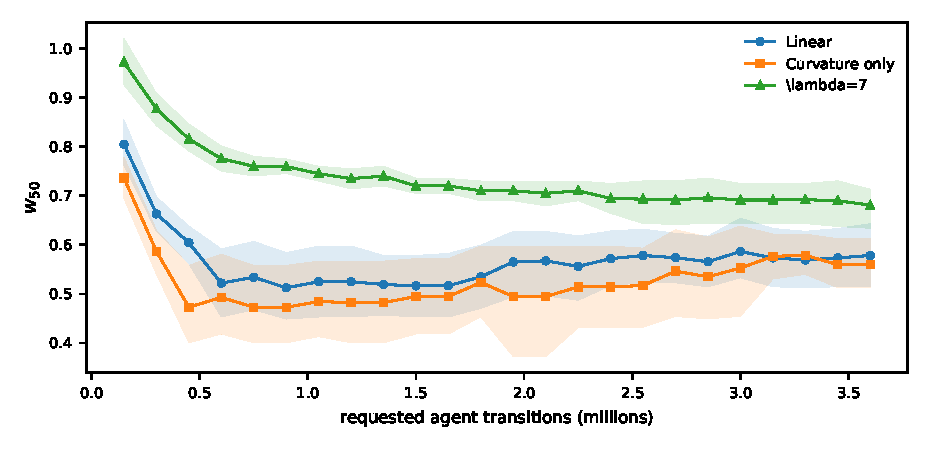
\includegraphics[width=.78\textwidth]{generated/v4/horizon_curves.pdf}
\caption{E3 crossings at every checkpoint (lines) with pointwise 95\% seed-block bands. Nine mixture cells, ten seeds per cell and condition.}
\label{fig:horizon}
\Description{Three crossing curves over training budget: lambda seven decreasing throughout; linear and curvature-only falling to 900k and rising afterwards.}
\end{figure}

% =======================================================================
\section{Reward-Transform Comparisons}
\label{sec:transforms}

\paragraph{The loss multiplier opposes curvature.}
In the legacy decomposition at 300k (20 seeds per cell), the linear null gives \RepeatedNull{}, curvature
alone ($\alpha{=}\beta{=}0.88$, the conventional prospect-theory estimate~\citep{tversky1992}, not tuned)
lowers the crossing to 0.585 ($-0.100$ $[-0.145,-0.057]$ vs.\ linear), and raising $\lambda$ from 1 to 7
raises it to \HighLambda{} (Figure~\ref{fig:decomposition}; per-$\lambda$ values in
Appendix~\ref{app:estimation}). Reported as a single ``prospect-theoretic'' treatment the two effects
partially cancel. Against the curvature baseline the loss-multiplier shift is \LossMultiplierShift{}.
On its own, this shift cannot distinguish loss asymmetry from the larger reward magnitude the multiplier
creates; Section~\ref{sec:optimizer} separates the two.

\begin{figure}[!htbp]
\centering
\includegraphics[width=.92\textwidth]{generated/decomposition_observed.pdf}
\caption{Legacy supply PPO null and selected transform conditions at 300k. Points show collapse counts divided by cell totals with 95\% Wilson intervals; curves are Firth fits over observed grids. Vertical bands are midpoint seed-block intervals.}
\label{fig:decomposition}
\Description{Four panels compare observed collapse proportions and fitted midpoints for null, lambda one, lambda three and lambda seven.}
\end{figure}

\begin{table*}[t]
\caption{Supply-PPO reward-transform decomposition at 300k requested agent transitions and descriptive equivalent linear-training budgets. Differences use paired seed-block draws. Equivalent budgets invert the four-point cross-sectional fit $w_{50}=1.4824-0.13748\ln(T/1000)$ and propagate the same 2,000 bootstrap replicates; they are descriptive, not causal. $\dagger$ denotes extrapolation below the observed 150k--900k horizon range.}
\label{tab:decomposition}
\centering\small
{\setlength{\tabcolsep}{4pt}
\begin{tabular}{@{}lllll@{}}
\toprule
Condition & Crossing and 95\% CI & Versus null & Versus curvature & Equivalent budget, k \\
\midrule
Linear null & $0.685$ $[0.650,0.715]$ & -- & -- & $330$ $[275,406]$ \\
Curvature ($\lambda=1$) & $0.585$ $[0.544,0.624]$ & $-0.100$ $[-0.145,-0.057]$ & -- & $685$ $[535,942]$ \\
$\lambda=3$ & $0.775$ $[0.755,0.790]$ & $+0.090$ $[+0.065,+0.115]$ & $+0.190$ $[+0.150,+0.229]$ & $172$ $[140,211]$ \\
$\lambda=7$ & $0.852$ $[0.840,0.865]$ & $+0.167$ $[+0.134,+0.203]$ & $+0.268$ $[+0.230,+0.306]$ & $98$ $[67,128]$$^{\dagger}$ \\
\bottomrule
\end{tabular}
}
\end{table*}


\paragraph{Equivalent linear-training budget.}
As a descriptive translation, inverting the legacy cross-sectional fit
$w_{50}=1.4824-0.13748\ln(T/1000)$ maps curvature-only at 300k to a linear budget of 685k $[535,942]$
and $\lambda=7$ to 98k $[67,128]$ (an extrapolation below the observed 150k--900k range); the repeated
linear null maps to 330k $[275,406]$ (Table~\ref{tab:decomposition}). This mapping is not causal,
but it anticipates the next section: under the default optimizer the loss multiplier behaves like a
smaller training budget.

% =======================================================================
\section{The Default Optimizer Masks the Asymmetric Effect}
\label{sec:optimizer}

\paragraph{Design (E1, E2).}
The pre-registered factorial crosses two optimizer modes with two reward modes at 300k. The optimizer
modes are SB3's default global clip and separate actor and critic Adam optimizers without clipping. The
reward modes are raw transformed rewards and online normalization (\texttt{VecNormalize} of rewards by
the running standard deviation of discounted returns, no observation normalization). Each cell runs the
four arms B, A, S and R on eight mixture cells $\{0,.2,.4,.5,.6,.7,.85,1\}$ with seeds 42--51, for
1,280 trajectories. An addendum (E2, 320 trajectories) keeps the default clip and raw rewards but sets
Adam's $\epsilon$ to $10^{-8}$. The pre-declared readings were: an A$-$S interval excluding zero after
both interventions indicates a sign-asymmetric effect; collapse of the symmetric contrasts after an
intervention indicates a scale or optimizer mechanism.

\paragraph{Under the default configuration, symmetric scaling mimics loss asymmetry.}
In the default cell every minibatch exceeds the clip norm, and the critic's pre-clip gradient norm
grows from \VfourCriticNormB{} (B) to \VfourCriticNormS{} (S) while the actor's stays near 2. The applied
actor update after clipping is \VfourAppliedActorB{} for B and \VfourAppliedActorS{} for S
(Table~\ref{tab:factorial_diagnostics}). Symmetric $\times7$ scaling therefore moves the crossing by
\VfourSymStd{} relative to B, at least as far as the loss multiplier, and A$-$S is
\VfourAsymStd{} (Table~\ref{tab:factorial_contrasts}).

\paragraph{Removing the coupling removes the symmetric effect but not the asymmetric one.}
With normalized rewards the critic's gradient falls below the clip norm, the actor carries almost all
of the gradient energy, and the symmetric effects vanish (S$-$B \VfourSymNorm{}). With separate
optimizers alone the symmetric $\times7$ effect shrinks to \VfourSymSep{} and the $\times3.451$ effect
vanishes. With both interventions, S$-$B is \VfourSymBoth{}, while A$-$B remains \VfourLossBoth{}. The
asymmetric contrast A$-$S is positive and excludes zero under normalization (\VfourAsymNorm{}), separate
optimizers (\VfourAsymSep{}) and both together (\VfourAsymBoth{}), so the pre-declared criterion for a
sign-asymmetric effect is met. The changes in each contrast relative to the default cell are in
Table~\ref{tab:factorial_interactions}; Figure~\ref{fig:factorial} summarizes them.

\paragraph{The artifact acts through critic target magnitude, not Adam's $\epsilon$.}
Lowering $\epsilon$ to $10^{-8}$ leaves the symmetric effect in place (S$-$B \VfourSymEps{}; change
relative to default \VfourSymEpsChange{}), contrary to our pre-declared alternative that the clipped
actor gradients were being suppressed by Adam's $\epsilon$ floor. Normalizing rewards, which bounds the
critic's targets, removes the effect, whereas separating the optimizers only reduces it, consistent with
a larger critic target slowing value learning even without clipping.

\paragraph{The baseline crossing itself depends on the optimizer.}
The curvature-only crossing B is \VfourBaselineStd{} in the default cell and \VfourBaselineRange{} in
the other cells (Table~\ref{tab:factorial_crossings}). An absolute $\wcrit$ is therefore a property of
the learner's optimizer configuration as well as of the reward design; comparisons are valid only
within a fixed configuration.

\begin{table}[!htbp]
\caption{Optimizer $\times$ reward-normalization factorial (E1) and Adam-$\epsilon$ addendum (E2): crossings $w_{50}$ at 300k with 95\% seed-block intervals. B: curvature only; A: losses $\times7$; S: both branches $\times7$; R: both branches $\times3.451$ (A's pooled RMS ratio). Ten seeds per cell, eight mixture cells, one platform.}
\label{tab:factorial_crossings}
\centering\footnotesize
\begin{tabular}{@{}lcccc@{}}
\toprule
Optimizer / reward & B & A & S & R \\
\midrule
Global clip, raw (default) & \begin{tabular}[t]{@{}c@{}}$0.538$\\[-1pt]{\scriptsize $[0.461,\,0.624]$}\end{tabular} & \begin{tabular}[t]{@{}c@{}}$0.821$\\[-1pt]{\scriptsize $[0.775,\,0.864]$}\end{tabular} & \begin{tabular}[t]{@{}c@{}}$0.895$\\[-1pt]{\scriptsize $[0.835,\,0.957]$}\end{tabular} & \begin{tabular}[t]{@{}c@{}}$0.794$\\[-1pt]{\scriptsize $[0.775,\,0.821]$}\end{tabular} \\
Global clip, normalized reward & \begin{tabular}[t]{@{}c@{}}$0.306$\\[-1pt]{\scriptsize $[0.201,\,0.413]$}\end{tabular} & \begin{tabular}[t]{@{}c@{}}$0.593$\\[-1pt]{\scriptsize $[0.527,\,0.655]$}\end{tabular} & \begin{tabular}[t]{@{}c@{}}$0.356$\\[-1pt]{\scriptsize $[0.272,\,0.436]$}\end{tabular} & \begin{tabular}[t]{@{}c@{}}$0.367$\\[-1pt]{\scriptsize $[0.324,\,0.414]$}\end{tabular} \\
Separate optimizers, raw & \begin{tabular}[t]{@{}c@{}}$0.326$\\[-1pt]{\scriptsize $[0.256,\,0.392]$}\end{tabular} & \begin{tabular}[t]{@{}c@{}}$0.661$\\[-1pt]{\scriptsize $[0.628,\,0.696]$}\end{tabular} & \begin{tabular}[t]{@{}c@{}}$0.487$\\[-1pt]{\scriptsize $[0.412,\,0.569]$}\end{tabular} & \begin{tabular}[t]{@{}c@{}}$0.353$\\[-1pt]{\scriptsize $[0.270,\,0.442]$}\end{tabular} \\
Separate optimizers, normalized & \begin{tabular}[t]{@{}c@{}}$0.414$\\[-1pt]{\scriptsize $[0.351,\,0.506]$}\end{tabular} & \begin{tabular}[t]{@{}c@{}}$0.602$\\[-1pt]{\scriptsize $[0.560,\,0.641]$}\end{tabular} & \begin{tabular}[t]{@{}c@{}}$0.365$\\[-1pt]{\scriptsize $[0.282,\,0.439]$}\end{tabular} & \begin{tabular}[t]{@{}c@{}}$0.350$\\[-1pt]{\scriptsize $[0.252,\,0.438]$}\end{tabular} \\
Global clip, raw, Adam $\epsilon{=}10^{-8}$ & \begin{tabular}[t]{@{}c@{}}$0.450$\\[-1pt]{\scriptsize $[0.387,\,0.534]$}\end{tabular} & \begin{tabular}[t]{@{}c@{}}$0.757$\\[-1pt]{\scriptsize $[0.729,\,0.775]$}\end{tabular} & \begin{tabular}[t]{@{}c@{}}$0.708$\\[-1pt]{\scriptsize $[0.649,\,0.770]$}\end{tabular} & \begin{tabular}[t]{@{}c@{}}$0.615$\\[-1pt]{\scriptsize $[0.559,\,0.683]$}\end{tabular} \\
\bottomrule
\end{tabular}
\end{table}

\begin{table}[t]
\caption{Paired seed-block contrasts within each optimizer cell. $^{\ast}$: 95\% interval excludes zero. A$-$S is the pre-declared asymmetry contrast; S$-$B and R$-$B are symmetric-scaling effects.}
\label{tab:factorial_contrasts}
\centering\scriptsize
\resizebox{\linewidth}{!}{%
\begin{tabular}{@{}lcccc@{}}
\toprule
Optimizer / reward & A$-$S & A$-$B & S$-$B & R$-$B \\
\midrule
Global clip, raw (default) & $-0.074$ $[-0.150,\,+0.000]$ & $+0.283$$^{\ast}$ $[+0.181,\,+0.386]$ & $+0.357$$^{\ast}$ $[+0.249,\,+0.464]$ & $+0.256$$^{\ast}$ $[+0.160,\,+0.344]$ \\
Global clip, normalized reward & $+0.237$$^{\ast}$ $[+0.169,\,+0.305]$ & $+0.287$$^{\ast}$ $[+0.199,\,+0.386]$ & $+0.050$ $[-0.035,\,+0.144]$ & $+0.060$ $[-0.068,\,+0.179]$ \\
Separate optimizers, raw & $+0.174$$^{\ast}$ $[+0.083,\,+0.255]$ & $+0.334$$^{\ast}$ $[+0.274,\,+0.405]$ & $+0.160$$^{\ast}$ $[+0.078,\,+0.254]$ & $+0.027$ $[-0.024,\,+0.069]$ \\
Separate optimizers, normalized & $+0.237$$^{\ast}$ $[+0.136,\,+0.346]$ & $+0.188$$^{\ast}$ $[+0.082,\,+0.266]$ & $-0.049$ $[-0.117,\,+0.017]$ & $-0.064$ $[-0.176,\,+0.024]$ \\
Global clip, raw, Adam $\epsilon{=}10^{-8}$ & $+0.048$ $[-0.013,\,+0.111]$ & $+0.307$$^{\ast}$ $[+0.224,\,+0.363]$ & $+0.258$$^{\ast}$ $[+0.187,\,+0.330]$ & $+0.165$$^{\ast}$ $[+0.109,\,+0.219]$ \\
\bottomrule
\end{tabular}
}
\end{table}


\begin{figure}[!htbp]
\centering
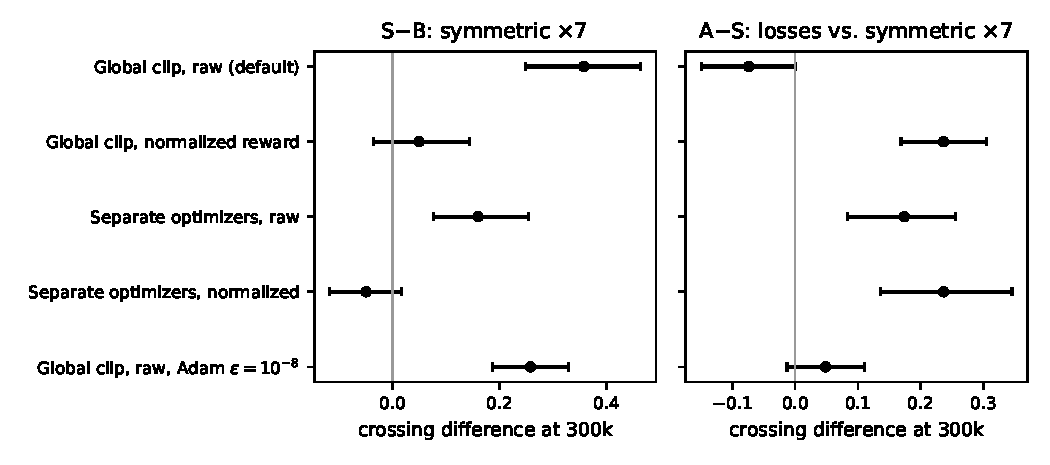
\includegraphics[width=\textwidth]{generated/v4/factorial_contrasts.pdf}
\caption{Symmetric-scaling (left) and asymmetric-minus-symmetric (right) crossing differences in each optimizer cell, with paired 95\% seed-block intervals. Under the default configuration (top row) symmetric scaling moves the crossing as far as the loss multiplier; with normalized rewards and/or separate optimizers it does not, while A$-$S becomes positive.}
\label{fig:factorial}
\Description{Two dot-and-interval panels across five optimizer cells. Symmetric effects are large in the default cell and near zero under normalization; asymmetric-minus-symmetric differences are near zero by default and positive under the interventions.}
\end{figure}

% =======================================================================
\FloatBarrier
\section{A Second Environment: Level-Based Foraging}
\label{sec:lbf}

\paragraph{Design (E4).}
We repeated the arm comparison with centralized-critic MAPPO~\citep{yu2022surprising} on Level-Based
Foraging~\citep{christianos2020shared} (5$\times$5 grid, two players, two foods), using the same SB3
update with a global clip or with separate optimizers. The local reward is the native food share minus
an effort cost of 0.02 per LOAD attempt; the team reward sums native food rewards; collapse is a native
team return below 0.626 over ten evaluation episodes, which never includes the effort cost. The arms are
linear, curvature only, A ($\lambda=4$) and S (both branches $\times4$), on ten mixture cells with ten
seeds and 2M timesteps (800 trajectories).

\paragraph{The asymmetric contrast replicates under both optimizers.}
The loss-only multiplier raises the crossing relative to symmetric scaling by \VfourLBFAsymGlobal{} with
the global clip and \VfourLBFAsymSep{} with separate optimizers (Table~\ref{tab:lbf}); the difference
between the two optimizer modes is not significant. Here, unlike the supply chain, the critic does not
dominate the clip: the actor carries \VfourLBFActorShare{} of the squared gradient norm in every arm.
The multiplier acts through the incentive structure instead. The loss branch is reached mainly through
the LOAD cost, so $\lambda$ multiplies the cost of the cooperative action, while S scales food rewards
and the cost together and leaves their ratio unchanged.

\paragraph{Two pre-declared predictions failed.}
We had predicted that curvature would raise the LBF crossing under the global clip and that separate
optimizers would shrink the curvature and symmetric shifts. Neither could be confirmed. The linear and
curvature arms rarely collapse at any $w$, so their crossings lie at or below the grid edge
(Table~\ref{tab:lbf}) and contrasts involving them are not identified. Both predictions also assumed
the supply-chain clipping pathway, which LBF does not exhibit.

\begin{table}[t]
\caption{MAPPO on Level-Based Foraging (E4): crossings and paired contrasts. Ten seeds, ten mixture cells, 2M timesteps, 800 trajectories. $^{\dagger}$: point estimate outside the sampled grid (linear and curvature rarely collapse, so their crossings are not localized). $^{\ast}$: interval excludes zero.}
\label{tab:lbf}
\centering\scriptsize
\resizebox{\linewidth}{!}{%
\begin{tabular}{@{}lcccccc@{}}
\toprule
Optimizer & Linear & Curvature & A & S & A$-$S & A$-$linear \\
\midrule
Global clip & $-0.289$ $[-1.333,\,-0.001]$$^{\dagger}$ & $-0.370$ $[-2.288,\,0.009]$$^{\dagger}$ & $0.525$ $[0.188,\,0.719]$ & $0.107$ $[-0.065,\,0.225]$ & $+0.418$$^{\ast}$ $[+0.218,\,+0.553]$ & $+0.814$$^{\ast}$ $[+0.422,\,+1.725]$ \\
Separate, no clip & $0.003$ $[-0.179,\,0.068]$ & $0.077$ $[-0.087,\,0.196]$ & $0.557$ $[0.250,\,0.724]$ & $0.077$ $[-0.126,\,0.237]$ & $+0.479$$^{\ast}$ $[+0.289,\,+0.613]$ & $+0.554$$^{\ast}$ $[+0.310,\,+0.718]$ \\
\bottomrule
\end{tabular}
}
\end{table}


% =======================================================================
\FloatBarrier
\section{Discussion and Limitations}
\label{sec:discussion}

A loss-only reward multiplier moves the coordination-collapse crossing in two environments, and once the
optimizer no longer converts reward scale into an actor learning-rate change, a symmetric multiplier
does not. Under SB3's default PPO configuration the same experiment yields the opposite conclusion. A
reward-design comparison that does not control critic scale can thus confuse an optimizer artifact with
a property of the reward. The asymmetric effect is a property of the transformed training signal, not
evidence about loss aversion as a psychological mechanism; in LBF it is plainly an incentive change on a
costly cooperative action.

\paragraph{Limitations.}
\begin{itemize}
\item \textbf{Budget.} No condition has a stable crossing by 3.6M, and the multiplier contrast shrinks
with budget; all readings are finite-budget.
\item \textbf{Optimizer and implementation.} Absolute crossings move with the optimizer configuration,
and all results use one PPO implementation (SB3 2.8.0); other implementations may couple actor and
critic differently.
\item \textbf{Environments.} Two environments and two learners, both small. In LBF only the loss-multiplier
arm has an interior crossing.
\item \textbf{Label and grid.} Crossings are conditional on the behavioral label and the sampled grid;
non-bracketed estimates are reported, not clipped.
\item \textbf{Platform.} Trained policies are not bit-reproducible across hardware and software builds;
labels and crossings are.
\item \textbf{Action representation.} An earlier ablation on the supply chain found no interior crossing
for PPO, QMIX or IQL on a coarse 11-level discretization of the base-stock action, so the phenomenon also
depends on the action representation.
\end{itemize}

A deployment requirement such as at most 5\% collapse would need its own probability target and
uncertainty assessment; the 50\% midpoint supplies no such guarantee.

% =======================================================================
\section{Conclusion}
\label{sec:conclusion}

Reward centralization is usually treated as a direction: more team signal helps. It also has a
measurable finite-budget location, $\wcrit$, that moves with reward transforms, training budget and the
optimizer. Measured with the optimizer coupling removed, a loss-only multiplier moves the crossing and a
symmetric multiplier does not, in two environments; measured with default settings, the two cannot be
told apart. We therefore recommend reporting $\wcrit$ together with the optimizer configuration and,
for any reward-transform comparison, a symmetric-scaling control run under value or reward
normalization.

% =======================================================================
\section*{Ethical Statement}

This work is entirely simulated, with no human subjects or personal data. Reported thresholds are
substrate-specific and must be re-measured before use.
